\documentclass[a4paper,11pt,twocolumn]{article}
\usepackage{icphs2015}
\usepackage{tipa}
\usepackage{colortbl}


\title{ACOUSTICS OF SPANISH AND ENGLISH CORONAL STOPS}
\author{Joseph V. Casillas, Yamile D\'{i}az and Miquel Simonet}
\organization{University of Arizona, Tucson}
\email{\{jvcasill, ydiaz44, simonet\}@email.arizona.edu}

\begin{document}

\maketitle

\begin{abstract}
This study explores the acoustic correlates that distinguish coronal stops (/t/, /d/) between English and Spanish. English and Spanish coronal stops are hypothesized to differ in terms of voice-onset time and place of articulation. We are particularly concerned with capturing the place of articulation difference with acoustic data, as the voice-onset time difference is well known. Specifically, we focus on English /d/ and Spanish /t/, which are phonetically-voiceless stops with a short-lag voice-onset time. Spanish \textipa{/t/} has been described as being articulated at dental place, whereas English \textipa{/d/} is articulated at alveolar place. Mixed-effects models explored various spectral measurements of the consonant burst and found that standard deviation, relative burst intensity, and center of gravity differed as a function of place of articulation (or language).
\end{abstract}

\keywords{Coronal stops, Spectral moments, VOT, Spanish, English}

\section{Introduction}

%Previous research attests that coronal place is the most common place of articulation for stops in the sound inventories of the world's languages \cite{henton_1992fk}.
Spanish and English both have coronal stops (/d, t/); however, their phonetic implementation differs. English /d/ and /t/ are produced with an alveolar place of articulation (POA) \cite{picard1987introduction}. Spanish /d/ and /t/, on the other hand, are both produced with a dental POA \cite{hualde2005sounds}. These descriptions rest mostly on impressionistic observations. This investigation sets out to explore the acoustic correlates related to place differences amongst these segments.

An important difference between Spanish and English has to do with their treatment of the stop voicing distinction common to these languages. Both distinguish between /t/ and /d/ by exploiting the acoustic correlate voice-onset time (VOT)---the acoustic output of the coordination of glottal and supra-glottal gestures that results in a time difference between the onset of modal voicing and articulatory release---; however, the manner in which they exploit VOT differs between the two languages. In English, /d/ has a short-lag VOT and /t/ has a long-lag VOT, whereas in Spanish /d/ has a lead VOT (prevoicing) and /t/ has a short-lag VOT \cite{liskerAbramson1964, williamsModification1979}.

The question of how bilinguals who speak Spanish and English use VOT to distinguish voiced and voiceless stops in their two languages has been investigated at length \cite{williamsPerception1977, williamsModification1979}; however, studies to date have overlooked the fact that bilinguals would need to produce a difference in POA, in addition to differently exploiting VOT, in order to avoid coalescing English and Spanish coronal stops. To date, few analyses have used acoustic measures to investigate differences in POA of coronal stops; two exceptions are \cite{sundara2005acoustic} and \cite{sundara2006bilingualism}.

The fact that both Spanish and English have short-lag, phonetically voiceless stops in their sound inventory (/t/ and /d/, respectively) begs the question as to whether these two segments can be distinguished by any acoustic measures.  Accounting for POA differences via acoustic metrics opens the door for new areas of research regarding bilingualism and second-language learning. Similarly to \cite{sundara2005acoustic}, the goal of the present study is to try to capture the hypothesized place difference between English and Spanish with acoustic data. The present study focuses on monolingual speakers of both languages. Our future goals include studying the behavior of Spanish-English bilinguals to determine whether they exploit the place differences between Spanish and English coronal stops, similarly to \cite{sundara2006bilingualism}.

The first four spectral moments---center of gravity (COG), standard deviation (SD), skewness (SK), and kurtosis (KT)---provide acoustic measurements related to the shape of a spectrum (i.e. how the energy is distributed across frequency bands) \cite{jones2013bloomsbury}. Various investigators have used spectral moments to distinguish between place differences in fricatives \cite{gordon2002cross,jongman2000acoustic}; however, \cite{sundara2005acoustic} is one of a reduced number of studies to use spectral moments in order to analyze place differences in stops. Specifically, Sundara examined coronal stops in French and English, which (similarly to Spanish and English) are realized with dental and alveolar place, respectively. Her investigation found differences between the two languages in relative burst intensity, COG, SD, and KT that were triggered by differences in POA. It remains an open question whether place differences between Spanish and English can be accounted for in the same manner.

\section{METHOD}

The goal of this investigation was to explore the acoustic correlates that differentiate Spanish from English coronal stops. We measured VOT, the first four spectral moments, and relative burst intensity (see below). After establishing the expected differences in terms of VOT, we focused on an analysis of only the two short-lag stops (English /d/ and Spanish /t/). Of particular interest was the relative importance of each of these spectral measures with regard to POA differences across the two languages.

\subsection{Speakers}
  
In order to address the aforementioned issues, we recorded the speech of 16 female participants. Eight were native Spanish speakers between the ages of 18 and 23, all of which were recruited from the \textit{Universitat de les Illes Balears} campus community and were born and raised on the island of Majorca, Spain. Eight were native English speakers and were undergraduate students at the University of Arizona, born and raised in the US Southwest. The Spanish speakers had studied some English in Spain, and the English speakers had studied some Spanish in the U.S., but none of the speakers were able to maintain a basic conversation in their ``second'' language.

\subsection{Materials and Procedure}

We devised a list of 48 target words, 24 in English and 24 in Spanish. The target words contained the voiced and voiceless coronal stops of both languages in word initial position. For each language there was a total of 24 words, 12 beginning with /d/ and 12 beginning with /t/, equally divided between stressed and unstressed syllables. All stops were followed by a low vowel (/a/ for Spanish and /\ae, \textscripta/ for English). (See \cite{sundara2005acoustic}.)

In order to collect the acoustic data we used the ``delayed repetition technique'' widely used in bilingual-speech research \cite{flege1995}. The materials were read by 6 male native speakers of these languages: 3 native English speakers (recorded in Austin, Texas) and 3 native Spanish speakers (recorded on Majorca, Spain). These acoustic materials were used as auditory stimuli to be repeated outloud by the 16 female speakers whose speech is analyzed here.

The speakers produced the target words in the carrier phrase ``\_ is the word'' or the Spanish equivalent (``\_ es la palabra''). All words not containing coronal stops were considered distractors. The computer program Praat \cite{Praat} presented the sentences randomly in auditory form and the speakers were asked to listen to the entire sentence and then repeat it outloud after a beep at their own pace. They were not asked to imitate the voices of the male talkers, but to produce the sentences in their ``own way.''

The English data were recorded in a sound attenuated booth on the campus of the University of Arizona. The Spanish data were obtained in a quiet classroom on the campus of the \textit{Universitat de les Illes Balears}. In order to carry out the recordings we used a Shure SM10A dynamic head-mounted microphone, a Sound Devices MM-1 microphone pre-amplifier and a Marantz PMD660 digital speech recorder. The signal was digitized at 44.1 kHz and 16-bit quantization.

Each participant provided the dataset with 72 coronal stops (24 target words $\times$ 3 repetitions). Thus, a total of 1,152 tokens were recorded (24 words $\times$ 3 repetitions $\times$ 16 participants = 1,152 stops). Our initial analysis of VOT utilizes the entire dataset; however, for subsequent analyses of burst measurements we took a subset of this data (exactly half) containing only Spanish /t/ and English /d/, as these are the stops that are not easily be distinguished by VOT. Five tokens were removed due to mispronunciations or extraneous noise leaving a total of 571 tokens for burst analyses.

\subsection{Measurements}

The digitized sound files were low-pass filtered at 11.025 kHz. For each of the coronal stops, synchronized waveform and spectrographic displays were used to mark the onset of modal voicing and of the burst. The onset of voicing was taken to be the upwards zero-crossing of the first periodic pattern found in the oscillogram \cite{lieberman1988speech}. Voice-onset time was calculated as the difference (in ms) between the onset of modal voicing and the onset of the burst.

Unlike in \cite{sundara2005acoustic}, the duration of the burst was determined semi-automatically. For short-lag stops, the burst was equal to the duration of VOT (see above). Thus, in cases in which VOT was positive but smaller than 25 ms, the burst was variable. For stops with long-lag and lead VOT, the burst was exactly 25 ms. That is, the onset of the burst was determined by hand, but the offset of the burst was set to occur 25 ms after the onset---i.e., the longest bursts were 25 ms.

In order to calculate relative burst intensity (RI), we extracted the intensity of the burst (in dB), as well as the mean intensity of the following vowel, which was also manually segmented. RI was the difference between the intensity of the vowel and the intensity of the burst. All spectral measures (COG, SD, SK, KT) were derived from the spectral envelope (which ranged from 60 Hz to 11.025 kHz.). Tokens for which a clear burst could not be established were removed.

\subsection{Statistical analyses}

A linear mixed-effects model was fit to each acoustic measure detailed above (i.e. VOT, RI, COG, SD, SK, and KT). The analysis of VOT included the entire dataset. Language (Spanish, English) and consonant (/d/, /t/) were fixed effects. Individual speaker and word items were random effects \cite{Baayen:2008bd}, with random slopes for subjects and items for the effect consonant \cite{Barr:2013eh}. Statistical significance of group, consonant, and the group by consonant interaction were assessed using hierarchical partitioning of variance via nested model comparisons. Simultaneous Tests for General Linear Hypotheses analyzed all pairwise comparisons using Tukey Contrasts with adjusted
p-levels.

Subsequent analyses of residualized burst measurements only included Spanish /t/ and English /d/ data. The present study was concerned with analyzing the acoustic correlates (aside from VOT) that could account for POA differences. Because all burst metrics are directly related to VOT, the effect of this variable was partialed out of the burst measurements as a method of reducing multi-collinearity between predictors. In order to accomplish this, separate models were fit with each burst measurement regressed on VOT. The residuals of these models were then used as the predictors for all analyses.\footnote{See \cite{fowler1984segmentation}, \cite{gow2003feature} and \cite{McMurray:2010ep} for discussion and examples of this approach.} Thus, each omnibus model directly compared Spanish /t/ to English /d/.\footnote{Degrees of freedom for hypothesis tests were derived using the Satterthwaite approximation as implemented in the \emph{lmerTest} package in R \cite{rcitation}.} In each case, individual speaker and word items were given random intercepts. We report marginal R$^2$ and conditional R$^2$ as an indication of goodness of fit for all models \cite{Nakagawa2013}. Marginal R$^2$ provides a measure of variance explained without mixed-effects and conditional R$^2$ includes them.

The second analysis explored the extent to which each of the acoustic measures could provide useful information about the POA of the phonetically voiceless segments. To this end, we divided the dataset into two subsets of Spanish /t/ and English /d/ stops: a training set, comprised of 75\% of the data, and a testing set, comprised of 25\% of the data. We then used RI, COG, SD, SK and KT as predictors in a forward selection logistic regression model in which phoneme identity (Spanish /t/, English /d/) was the criterion variable. Causal priority was given to the correlates found to best predict POA in \cite{sundara2005acoustic}. After building the model on the training subset, we used cross-validation to predict the identity of the stops in the testing subset.


\section{RESULTS}

\begin{figure*}[t!]
\caption{VOT and burst measures of Spanish and English coronals.\label{fig:all}}
\begin{center}
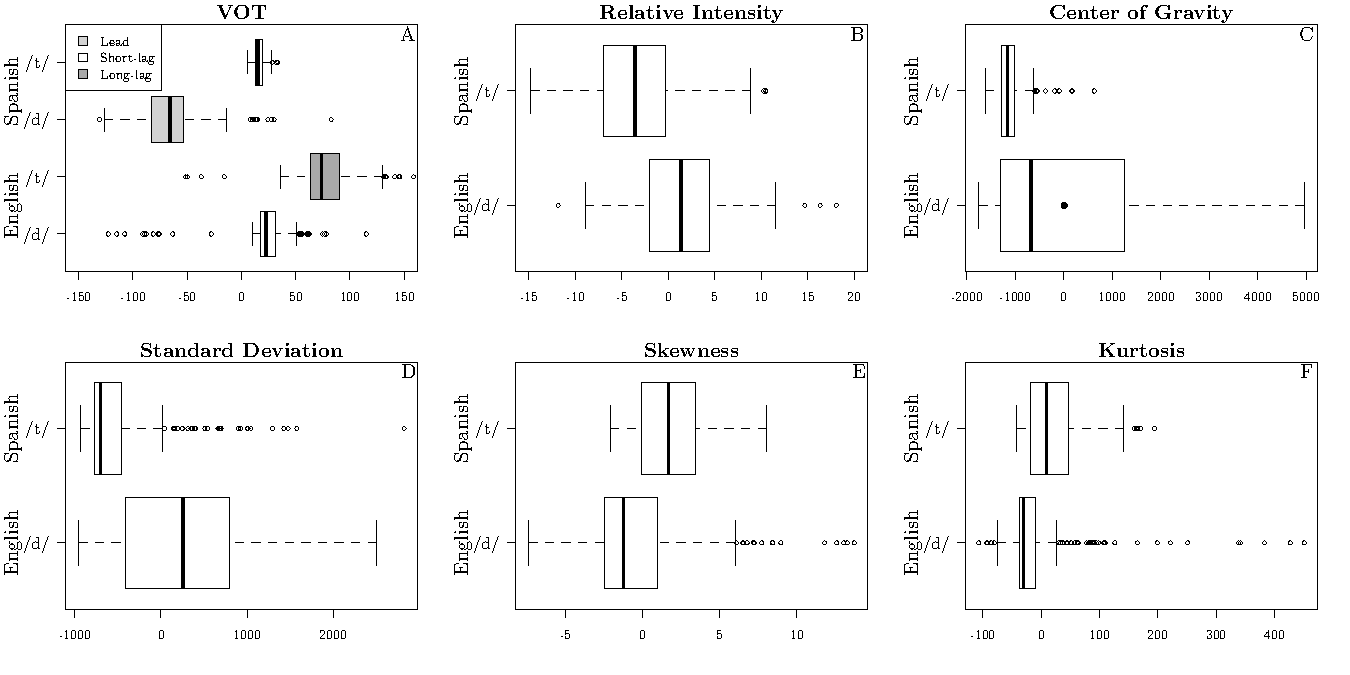
\includegraphics[width=.9\textwidth]{figures/prod.pdf}
\end{center}
\end{figure*}

\subsection{VOT}

The analysis of the VOT data revealed a main effect of language ($\chi$(2) = 44.07; p < 0.001), consonant ($\chi$(2) = 56.39; p < 0.001), as well as a language by consonant interaction ($\chi$(1) = 10.54; p < 0.002). Pairwise comparisons showed that all of the coronal stops differed from each other (p < 0.001), with the exception of the Spanish /t/ \textit{vs.} English /d/ short-lag stops. The mixed model provided the best fit for the data (conditional R$^2$ = 0.87; marginal R$^2$ = 0.82). Figure~\ref{fig:all}A plots VOT as a function of language and consonant. The light gray box shows that Spanish /d/ was produced with lead VOT ($\bar{x} = -64.48 \pm 28.56$ SD), and the dark gray box shows that English /t/ was produced with long-lag VOT ($\bar{x} = 77.63 \pm 25.63$ SD). The white boxes represent the short-lag stops of English and Spanish. VOT for English /d/ was slightly longer ($\bar{x} = 22.13 \pm 26.69$ SD) than Spanish /t/ ($\bar{x} = 16.18 \pm 5.08$ SD); however, this difference was negligible, likely due to the high rate of variability for English /t/. Thus, in these data VOT can account for differences between all coronal stops except for those that are manifested through short-lag VOT: English /d/ and Spanish /t/.

\subsection{Burst measurements}

Figure~\ref{fig:all}B plots RI of Spanish /t/ and English /d/. The data were best fit using the mixed-effects model (conditional R$^2$ = 0.66; marginal R$^2$ = 0.20). The analysis revealed that English /d/ was 4.81 dB $\pm 1.77$ standard errors (SE) higher that Spanish /t/ (t = -2.72; p < 0.02).

The COG data were also best fit using the mixed-effects model (conditional R$^2$ = 0.68; marginal R$^2$ = 0.19). Spanish /t/ was 1131 Hz $\pm$ 455 SE lower than the average English /d/ (t = -2.48, p < 0.03; see Figure~\ref{fig:all}C). Regarding SD, the mixed-effect model accounted for 61\% of the variance (vs. marginal R$^2$ of 26\%). The SD values for Spanish /t/ were 763 Hz $\pm$ 222 SE lower than English /d/ (t = -3.44, p < 0.004; see Figure~\ref{fig:all}D). The analysis of SK (Figure~\ref{fig:all}E) revealed that Spanish /t/ was 2.10 $\pm$ 0.87 SE units higher than English /d/ (t = 2.40; p < 0.03). Again, the data were best fit using the mixed effects model (conditional R$^2$ = 0.45; marginal R$^2$ = 0.12). Lastly, the KT data had the least amount of variance explained by the model (conditional R$^2$ = 0.26; marginal R$^2$ = 0.06). Spanish /t/ was 29.02 $\pm$ 14.30 se units higher than English /d/; however, this difference was not significant at our specified alpha level (t = 2.03, p = 0.06; see Figure~\ref{fig:all}F). In sum, all of the burst measurements, with the exception of kurtosis, differed as a function of language. This is taken as an indication that these metrics successfully accounted for place differences between the short-lag stops of English and Spanish.

The next step was to analyze the relative contribution of the burst measurements. The training subset of the data was analyzed via logistic regression, with the burst metrics as fixed effects for predicting the short-lag stop phoneme identity (Spanish /t/, English /d/). The model eliminated SK and KT from the analysis. Table~\ref{model_sum} summarizes the results. Nagelkerkes' pseudo R$^2$ is reported to give an indication of goodness-of-fit of each predictor as it was entered into the model. SD accounted for the largest amount of the variance (35\%), followed by RI (5\%) and COG (2\%).

\begin{table}[h]
\caption{Regression analysis of /d/-/t/.\label{model_sum}}
\begin{center}
\begin{tabular}{@{}lccrr@{}}
\hline \\ [-2ex]
Metric & \emph{R}$^2$ & \emph{R}$^2_{\ change}$ & \emph{$\chi^2_{\ change}$} & \emph{p-value} \\
\hline \\ [-2ex]
SD  & .353  & .353 & 175.39 & < 0.001 \\
COG & .376  & .023 &  14.01 & < 0.001 \\
RI  & .425  & .049 &  30.01 & < 0.001 \\
SK  & .426  & .001 &   0.08 & > 0.05  \\
KT  & .432  & .006 &   4.36 & < 0.04  \\
\hline
\end{tabular}
\end{center}
\end{table}

Finally, the best fit model was used to predict the identity of the short-lag stops of the testing subset. The model performed with 87\% accuracy (out of sample error = 0.13). That is, given the data for SD, RI and COG, it was possible to predict whether the stop was Spanish /t/ or English /d/ on 87\% of the testing subset (142 tokens).

\section{DISCUSSION AND CONCLUSION}

The results of the analyses showed that the phonetically voiceless coronal stops of English and Spanish can be distinguished by RI and by the spectral shape of the stop burst. Importantly, the present study indicates that the place of articulation differences described for Spanish /t/ and English /d/ are best accounted for using measures of SD, RI, and COG. SK and KT did not significantly contribute to predicting the POA of the short-lag stops in our data.

Our results partially corroborate the findings of \cite{sundara2005acoustic}. As is the case in the Canadian varieties of English and French investigated in \cite{sundara2005acoustic}, the two varieties of English and Spanish investigated here differ in place of articulation of their coronal stops---alveolar (English) and dental (French, Spanish), according to impressionistic descriptions. In our data, similar to \cite{sundara2005acoustic}, values of SD and other burst measures varied across the two languages; however, different from our findings, she also encountered significant differences for kurtosis.

The present study contributes language-specific acoustic characteristics of bursts in the short-lag coronal stops of two monolingual varieties of English and Spanish. Among other things, the findings provide base acoustic descriptions for future studies on Spanish-English bilinguals.

\newpage

\bibliographystyle{icphs2015}
\bibliography{vot}

\theendnotes


\end{document}
